\section*{Ziel}
    In diesem Versuch sollen grundlegende Schaltungen mit Operationsverstärkern aufgebaut und untersucht werden.
    Hierbei sollen Unterschiede zwischen einem realen und idealen Operationsverstärker, sowie einige Anwendungsmöglichkeiten und Grenzen verdeutlicht werden \cite{anleitung}.
\section{Theorie}
    \label{sec:theorie}
    \subsection{Operationsverstärker (OV)}
    Ein Operationsverstärker ist ein elektrisches Bauteil das hauptsächlich auf einem Differenzverstärker basiert.
    Der OV besitzt einen invertierten (-) und einen nicht invertierten (+) Eingang und gibt eine Ausgangsspannung aus die proportional zur Differenz des invertierten und nicht invertierten ist.
    Der Betrag der Ausgangsspannung des OV kann dabei maximal so grß wie die Betriebsspannung des OV's werden.

    Um einen Operationsverstärker zu beschreiben werden verschiedene definierende Größen verwendet.
    Ein idealer Operationsverstärker hat beispielsweise einen Eingangswiderstand $R_E$ von $\infty \; \si{\ohm}$ und einen Ausgangswiderstand $R_A$ von \SI{0}{\ohm}, diese Werte können bei realen OVs nicht erreicht werden und im Regelfall sind eher Werte wie $R_E > \SI{1}{\mega\ohm}$ und $R_A ≈ \num{10}-\SI{1000}{\ohm}$ zu erwarten.
    Die Verstärkung eines idealen OVs ist $V' = \frac{U_A}{U_E} ≈ \infty$ wobei typische Verstärkungen $V$ eines reellen OVs im Größenbereich \num{e4} bis \num{e6} liegen.
    Außerdem hängt das genaue Verhalten eines reellen OVs von vielen Parametern ab und er ist auf einen Frequenzbereich von \SI{10}{\hertz} bis \SI{10}{\kilo\hertz} beschränkt, wohingegen die Parameter beim idealen OV vernachlässigt werden und er über den kompletten Frequenzbereich arbeitet.
    \subsection{LM741}
        \begin{figure}[H]
            \centering
            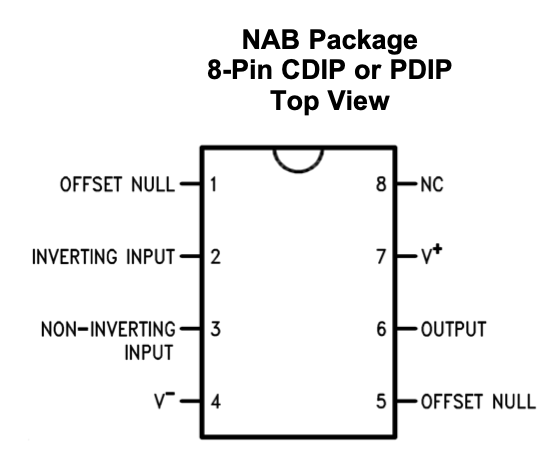
\includegraphics[width = 0.5\textwidth]{bilder/LM741.png}
            \caption{Ein Überblick über die Inputs des Operationsverstärkers LM741}
            \label{fig:LM741}
        \end{figure}
        Der LM741 OV besitzt 8 Kontakte für die verschiedenen Inputs des Verstärkers.
        Um mit dem Verstärker zu arbeiten sind vor allem die zwei Input Kontakte des invertierten Inputs an der Position 2 und des nicht invertierten Inputs an der Position 3 und der Output Kontakt an der Position 6 wichtig.
        Neben diesen Inputs und Outputs für das Verstärken besitzt das Bauteil noch mehrere für den Betrieb notwendige Kontakte.
        Auf Position 1 und 5 befindet sich jeweils ein 'Offset Null' Kontakt.
        Mit Kontakt 4 wird die Betriebsspannung für den invertierten Eingang und mit Kontakt 7 die für den nicht invertierten Eingang geliefert.
        Kontakt 8 ist 'No Connect' (NC) und hat keine Verwendung für den OV.
    \subsection{Invertierender-Linearverstärker}
        Im Versuch wird unter anderem mit einem Linearverstärker gearbeitet.
        Um die erwünschte Schaltung zu erreichen, wird der Ausgang des OV auf den invertierenden Eingang rückgekoppelt \ref{fig:inv_Ver}.
        Gemäß der großen Leerlaufverstärkung kann $U_N = 0$ angenommen werden.
        \begin{figure}[ht]
            \centering
            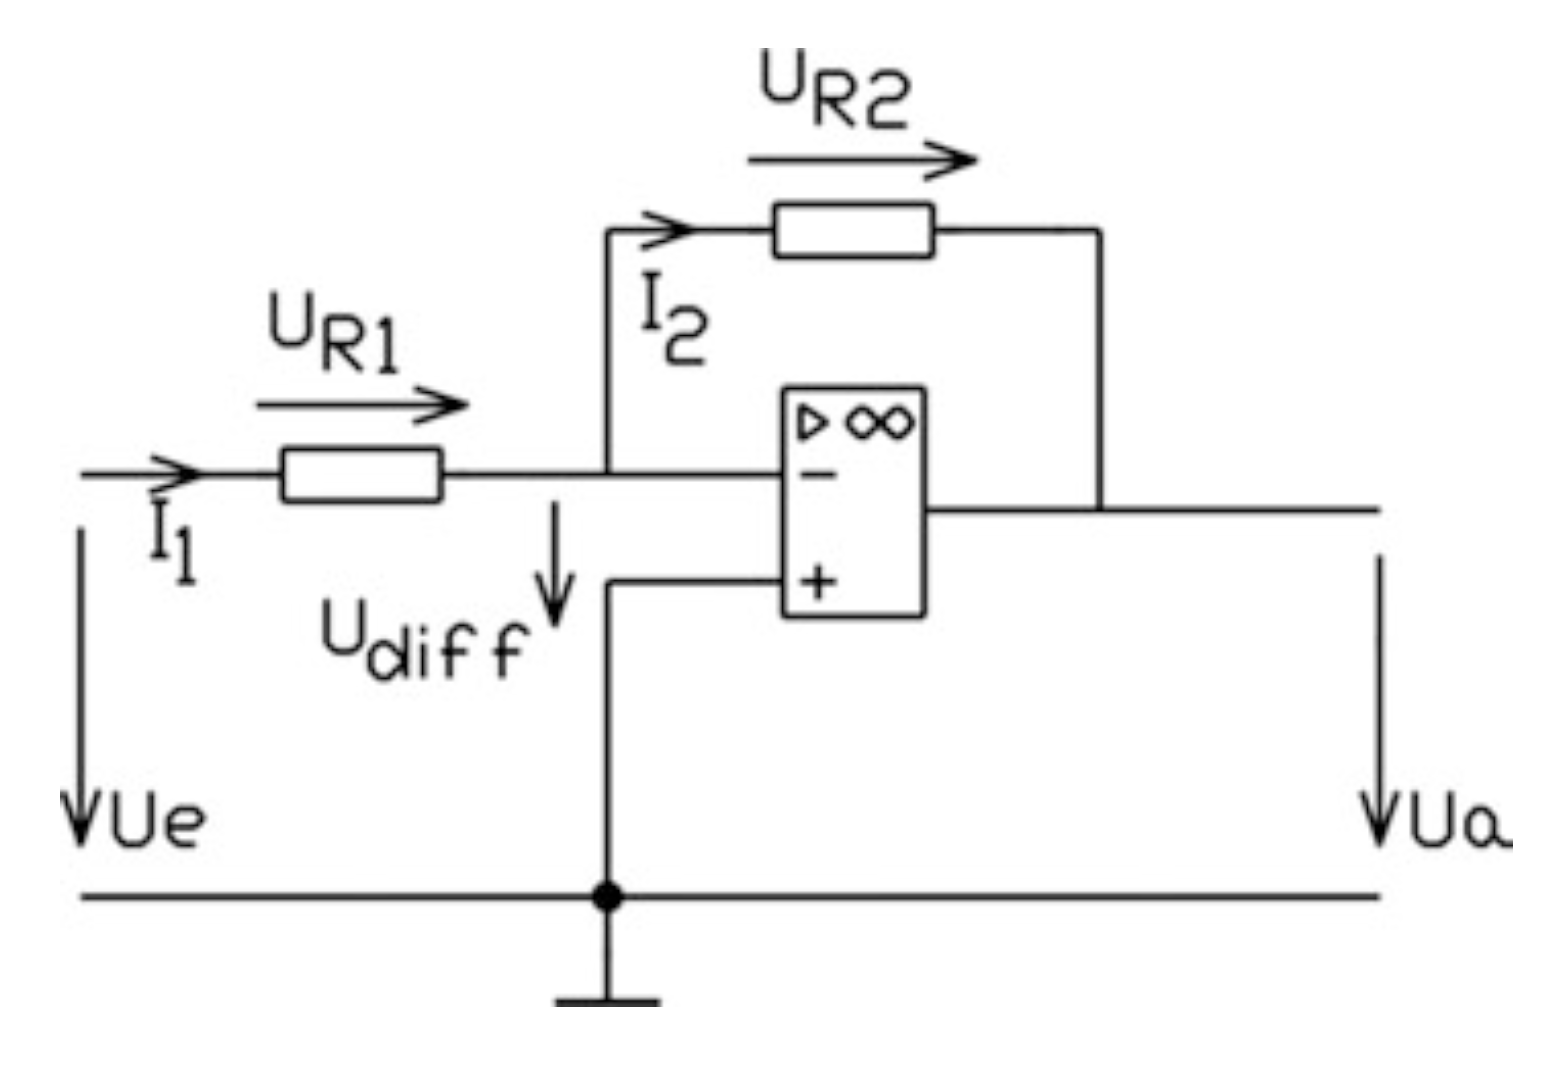
\includegraphics[width = 0.5\textwidth]{bilder/invertierender_verstaerker.png}
            \caption{Der Invertierende Verstärker entnommen aus Federau 2017}
            \label{fig:inv_Ver}
        \end{figure}
        Mithilfe der Maschenregel und der Knotenregel lässt sich dadurch die Verstärkung des invertierenden linearverstärkers in Abhängigkeit der Wiederstände bestimmen.
        \begin{align*}
            U_E -U_{R_1}-U_N = 0\\
            U_E -U_{R_1} = 0\\
            U_E = U_{R_1}
        \end{align*}
        Mit der Knotenregel zwischen $R_1$ und $R_2$ ergibt sich:
        \begin{align}
            I_1+I_2 = 0\nonumber\\
            \frac{U_{R_1}}{R_1} = -\frac{U_{R_2}}{R_2}\nonumber\\
            U_{R_2} = -\frac{R_2}{R_1} U_{R_1}\nonumber\\
            U_{A} = -\frac{R_2}{R_1} U_{E}\nonumber\\
            U_{A} = V' \cdot U_{E}\nonumber\\
            V' = \frac{U_A}{U_E} = -\frac{R_2}{R_1}
            \label{eqn:verstaerkung}
        \end{align}
        Mit der Annahme einer endlichen Leerlaufvertärkung ändert sich diese Formel für den realen OV zu:
        \begin{equation}
            \frac{1}{V'}= \frac{1}{V} +\frac{R_1}{R_2}
            \label{eqn:reale_verstaerkung}
        \end{equation}
    \subsection{Umkehr-Integrator}
    \label{sec:integrator}
        Um eine Integratorschaltung muss beim invertierenden Verstärker in der Rückkopplung lediglich der Widerstand mit einem Kondensator getauscht werden \ref{fig:integrator}.
        Die entstehende Schaltung kann nun das Eingangssignal integrieren.
        Der Kondensatorstrom über die Zeit integriert entspricht der Kapazität mit der angelegten Spannung multipliziert.
        Mithilfe der Knotenregel ergibt sich daher für den Knoten vor dem invertierenden Eingang:
        \begin{equation*}
            U_a = -\frac{1}{RC} \int U_1(t) dt
        \end{equation*}
        Daher wird wie zu sehen im Ausgangssignal das Eingangsignal integriert mit einem Faktor der antiproportional zum Widerstand und Kapazität ist.
        \begin{figure}[ht]
            \centering
            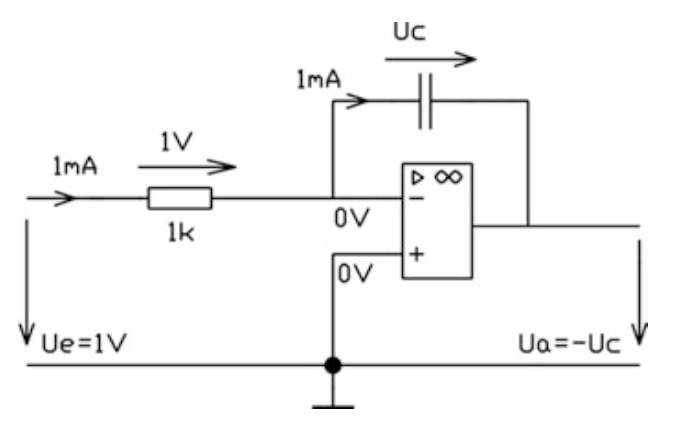
\includegraphics[width = 0.5\textwidth]{bilder/integrator.png}
            \caption{Der Integrator entnommen aus Federau 2017}
            \label{fig:integrator}
        \end{figure}
    \subsection{Invertierender-Differenzierer}
        Der invertierende Differenzierer ist aufgebaut wie der invertierende Linearverstärker, allerdings wird anstatt eines Widerstands im Eingangssignal ein Kondensator eingebaut \ref{fig:differenzierer}.
        Für die Ausgangsspannung des invertierenden Differenzierers ergibt sich:
        \begin{equation*}
            U_a = -RC \frac{dU_1}{dt}
        \end{equation*}
        Somit wird das differenzierte Eingangssignal mit einem Faktor proportional zu Kapazität und Widerstand ausgegeben.
        \begin{figure}[ht]
            \centering
            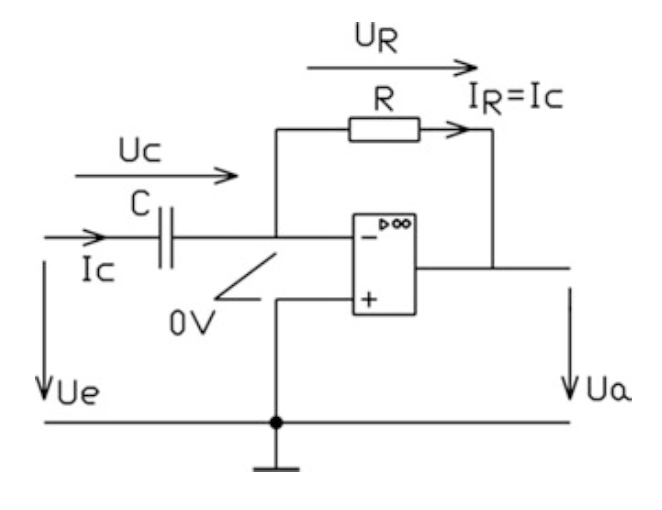
\includegraphics[width = 0.5\textwidth]{bilder/differenzierer.png}
            \caption{Der Differenzierer entnommen aus Federau 2017}
            \label{fig:differenzierer}
        \end{figure}
    \subsection{Nicht-invertierende-Schmitt-Trigger}
        Der nicht-invertierende Schmitt Trigger hat denselben Aufbau wie der invertierende Linearverstärker mit dem Unterschied dass in diesem Fall die Rückkopplung nicht auf den invertierenden sondern auf den nicht-invertierenden Eingang gelegt wird, dies ist eine sogenannte Mitkopplung \ref{fig:schmitt_trigger}.
        Mit der Schaltung des Schmitt Triggers kann der OV als Schalter genutzt werden.
        Immer wenn das Eingangsignal einen Schwellwert erreicht ändert sich das Ausgangssignal schlagartig zu einem von zwei festen Zuständen.
        Der Schwellwert $U_+$ ergibt sich zu:
        \begin{equation*}
            U_+  = \pm \frac{R_1}{R_2}U_B
        \end{equation*}
        mit der Betriebsspannung $U_B$. 
        Die beiden Zustände für das Ausgangssignal sind dabei $\pm U_B$.
        \begin{figure}[ht]
            \centering
            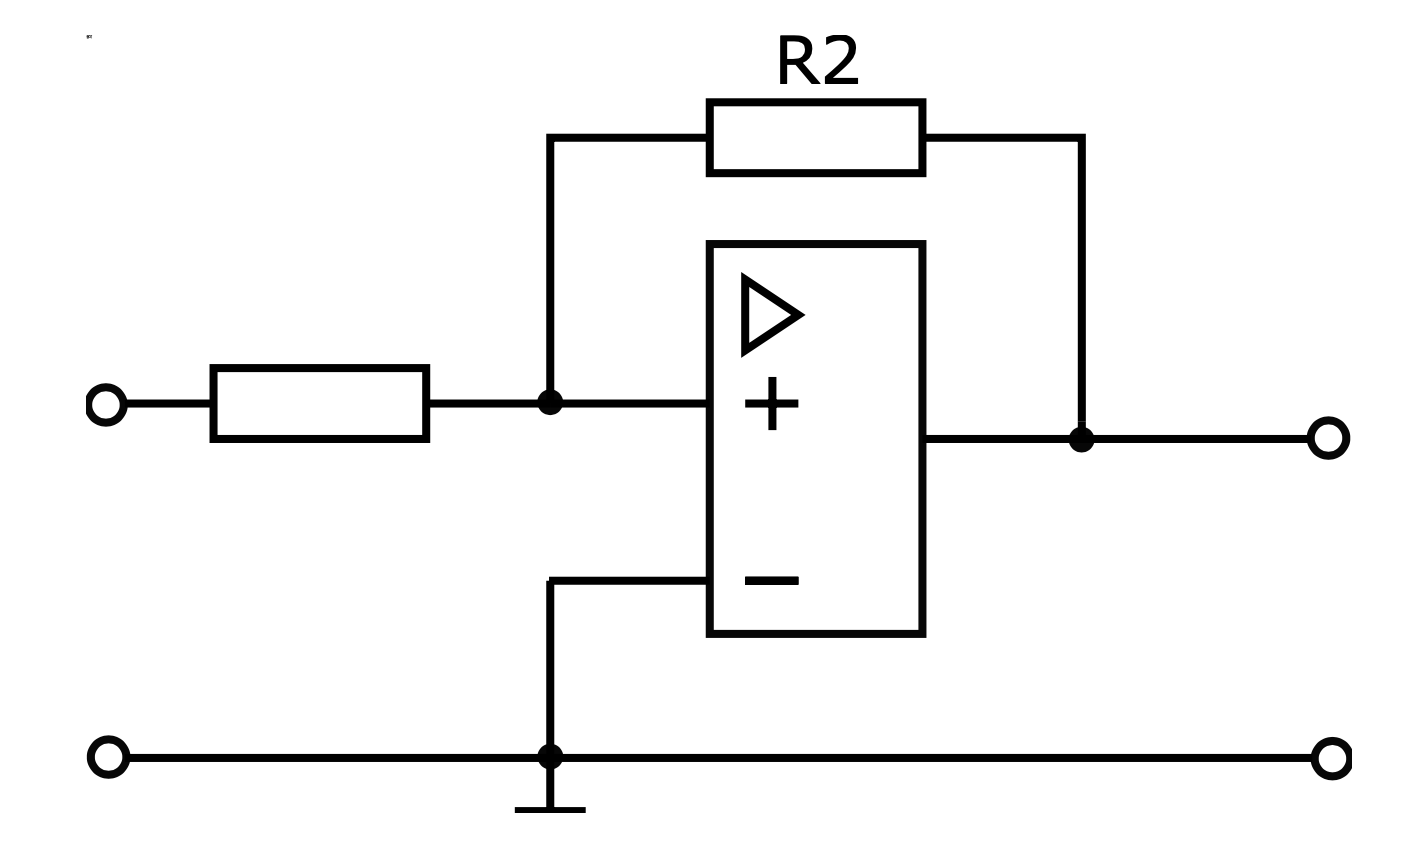
\includegraphics[width = 0.5\textwidth]{bilder/schmitt_trigger.png}
            \caption{Der Schmitt-Trigger entnommen aus der Versuchsanleitung}
            \label{fig:schmitt_trigger}
        \end{figure}
    \subsection{Signalgenerator}
        Der Signalgenerator entsteht wenn hinter der Schmitt Trigger Schaltung noch ein Integrator (\ref{sec:integrator}) geschaltet wird \ref{fig:signalgenerator}.
        Wenn nun die Ausgangsspannung des Schmitt Triggers (eine Rechtecksspannung) anschließend mit dem Integrator integriert wird ist es möglich mit dieser Schaltung ein Dreiecksspannungssignal zu erzeugen.
        \begin{figure}[ht]
            \centering
            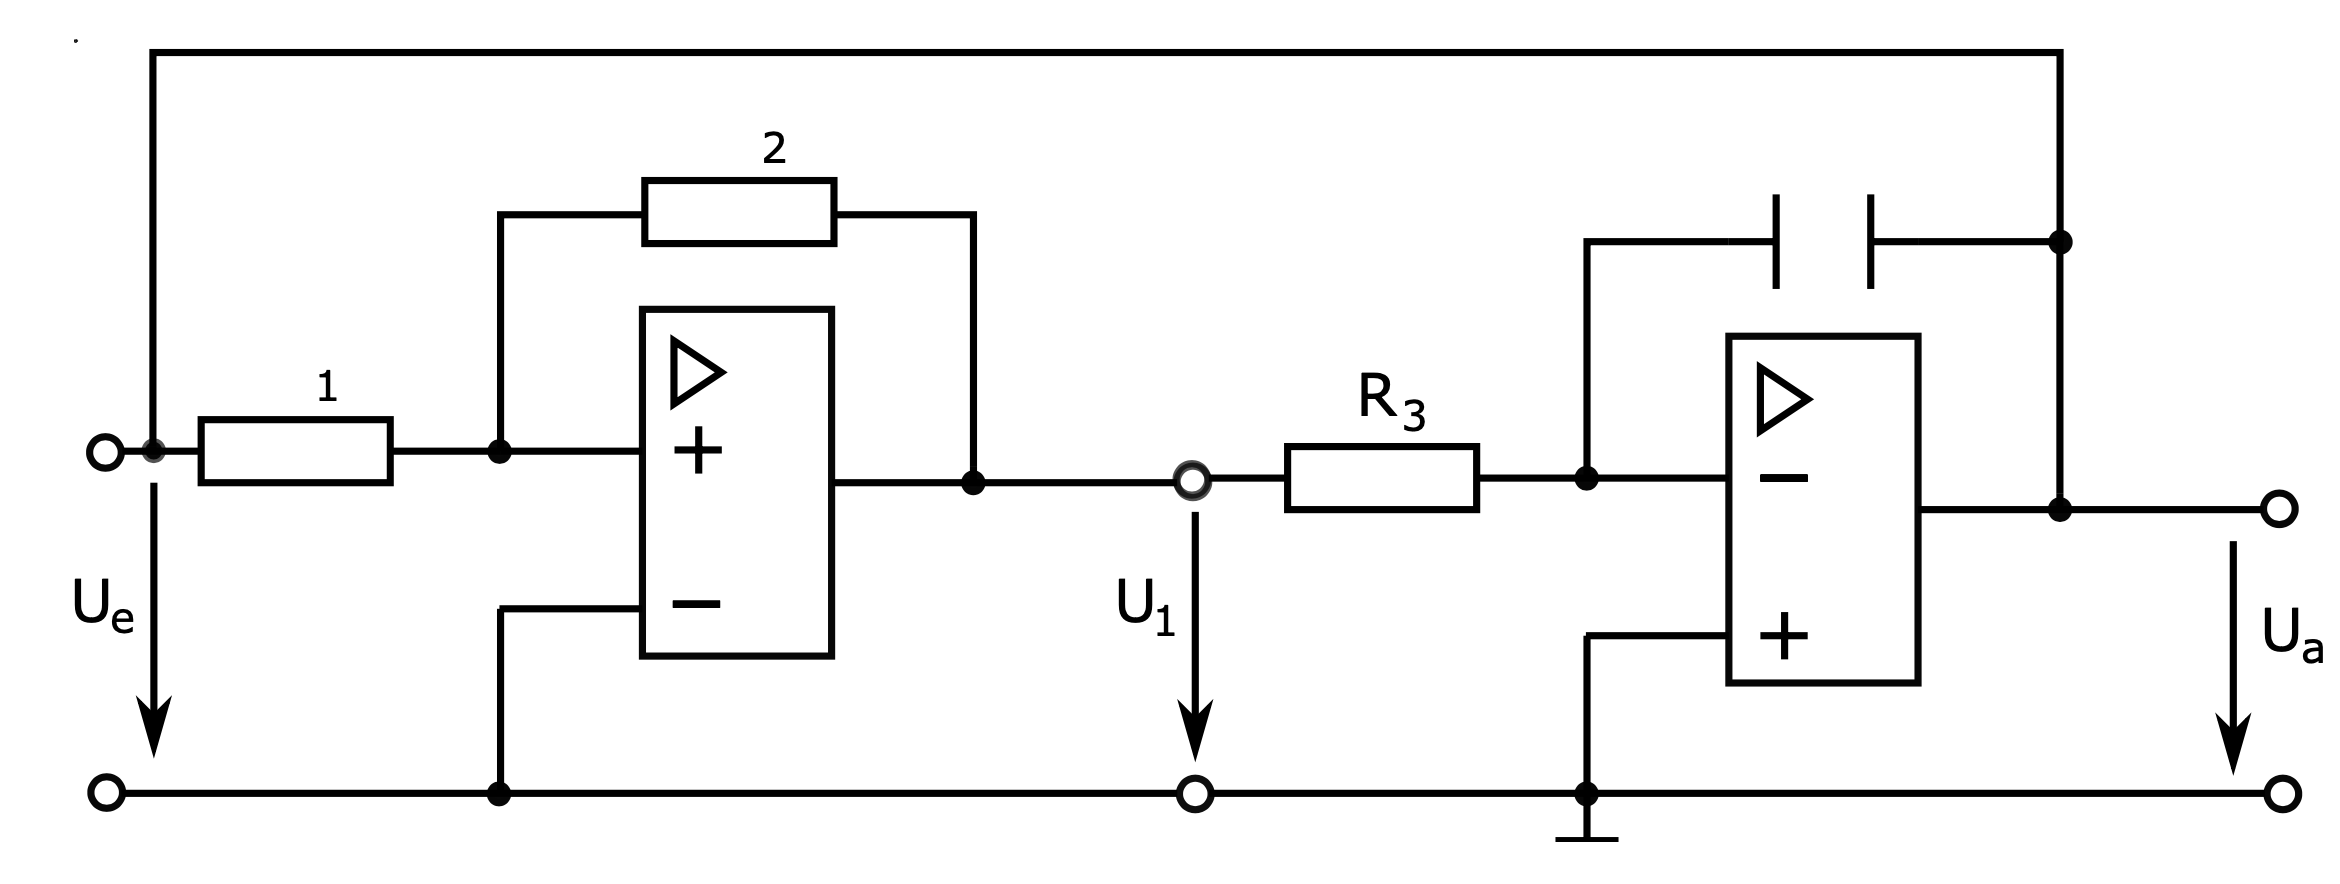
\includegraphics[width = 0.5\textwidth]{bilder/signalgenerator.png}
            \caption{Der Signalgenerator entnommen aus der Versuchsanleitung}
            \label{fig:signalgenerator}
        \end{figure}
    \subsection{Variierende Amplituden}
        Um eine Sinusspannung mit variierenden Amplituden zu erreichen wird die Schaltung gemäß Abbildung \ref{fig:variierende_Amp} aufgebaut.
        Die Schltung umfasst eine Verbindung von zwei Integratorschaltungen mit einem Invertierer.
        Durch diese Kombination von Schaltungen ist es möglich eine Sinusspannung zu erzeugen, dabei lässt sich durch das eingebaute Potentiometer dei Amplitude der Sinusspannung beeinflussen.
        \begin{figure}[ht]
            \centering
            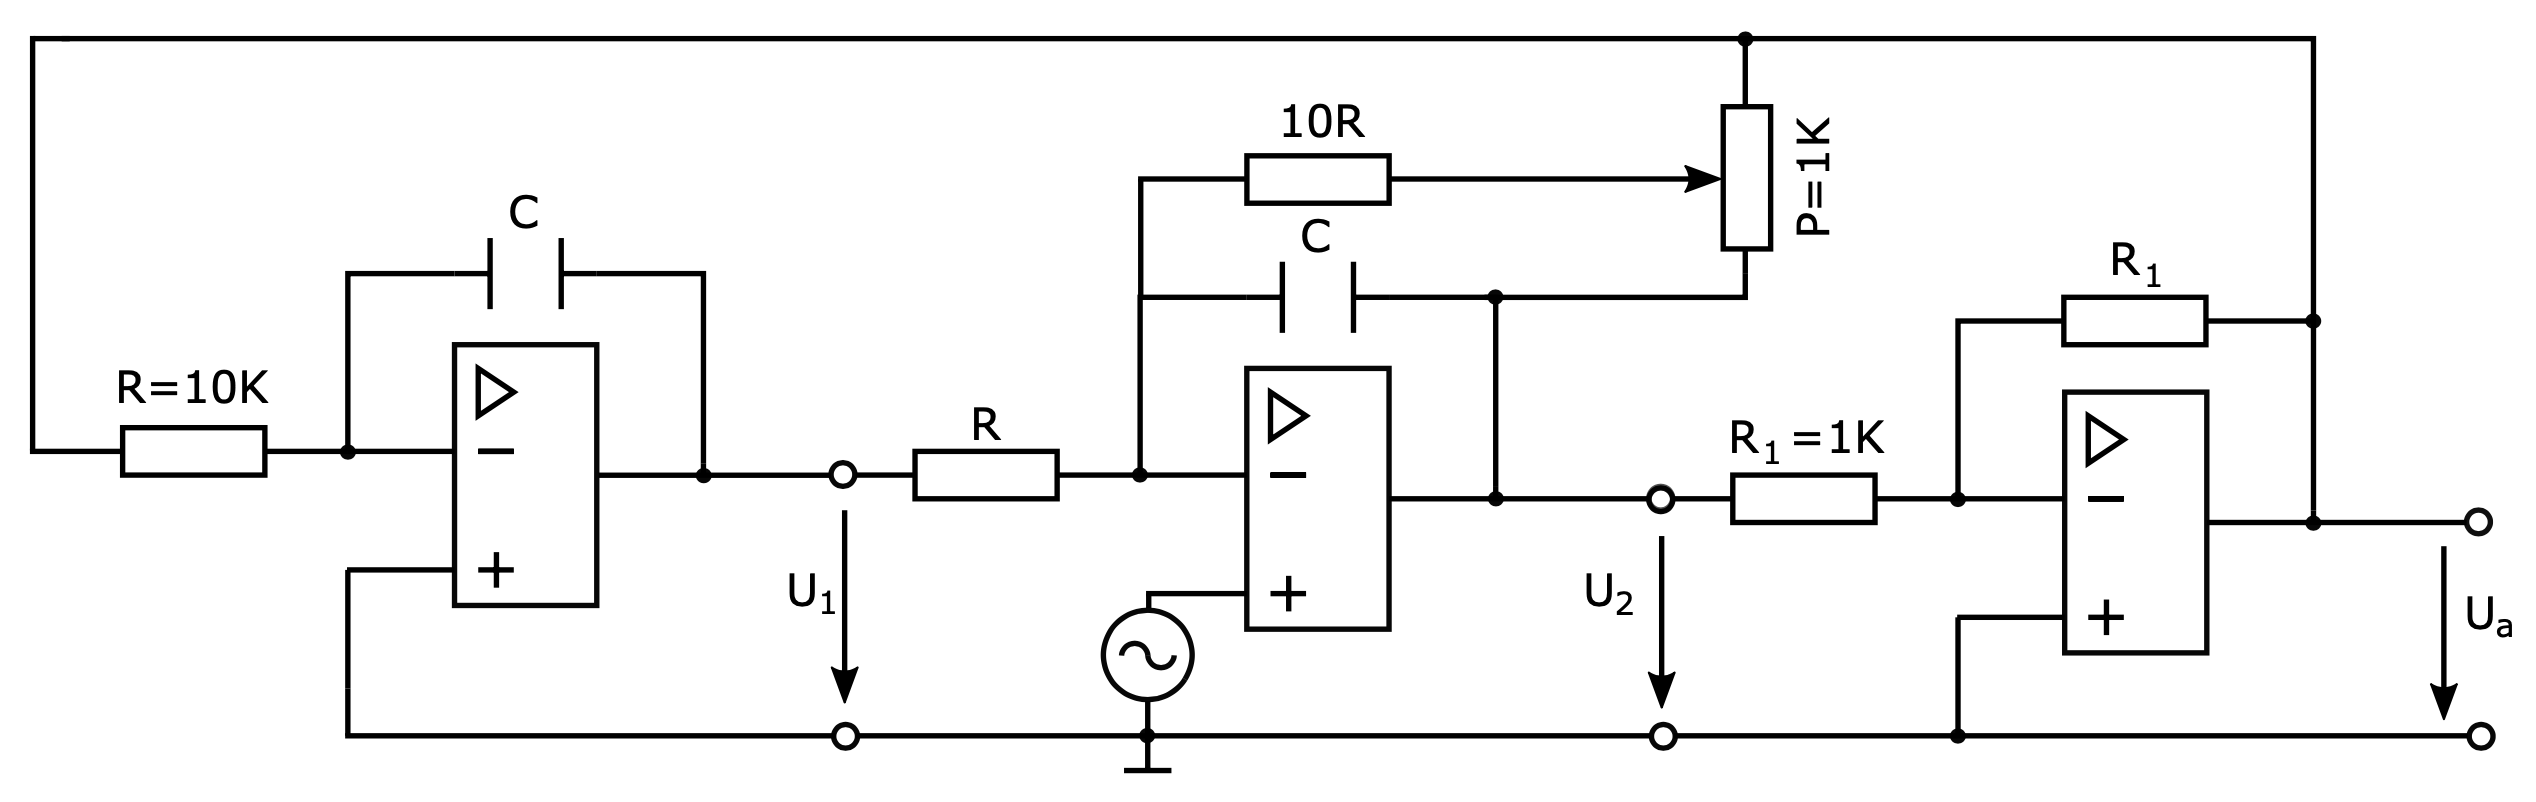
\includegraphics[width = 0.5\textwidth]{bilder/variierende_Amp.png}
            \caption{Die variierende Amplituden Schaltung entnommen aus der Versuchsanleitung}
            \label{fig:variierende_Amp}
        \end{figure}